\documentclass{ximera}

%\usepackage{todonotes}

\newcommand{\todo}{}

\usepackage{esint} % for \oiint
\ifxake%%https://math.meta.stackexchange.com/questions/9973/how-do-you-render-a-closed-surface-double-integral
\renewcommand{\oiint}{{\large\bigcirc}\kern-1.56em\iint}
\fi


\graphicspath{
  {./}
  {ximeraTutorial/}
  {basicPhilosophy/}
  {functionsOfSeveralVariables/}
  {normalVectors/}
  {lagrangeMultipliers/}
  {vectorFields/}
  {greensTheorem/}
  {shapeOfThingsToCome/}
  {dotProducts/}
  {partialDerivativesAndTheGradientVector/}
  {../productAndQuotientRules/exercises/}
  {../normalVectors/exercisesParametricPlots/}
  {../continuityOfFunctionsOfSeveralVariables/exercises/}
  {../partialDerivativesAndTheGradientVector/exercises/}
  {../directionalDerivativeAndChainRule/exercises/}
  {../commonCoordinates/exercisesCylindricalCoordinates/}
  {../commonCoordinates/exercisesSphericalCoordinates/}
  {../greensTheorem/exercisesCurlAndLineIntegrals/}
  {../greensTheorem/exercisesDivergenceAndLineIntegrals/}
  {../shapeOfThingsToCome/exercisesDivergenceTheorem/}
  {../greensTheorem/}
  {../shapeOfThingsToCome/}
  {../separableDifferentialEquations/exercises/}
  {vectorFields/}
}

\newcommand{\mooculus}{\textsf{\textbf{MOOC}\textnormal{\textsf{ULUS}}}}

\usepackage{tkz-euclide}
\usepackage{tikz}
\usepackage{tikz-cd}
\usetikzlibrary{arrows}
\tikzset{>=stealth,commutative diagrams/.cd,
  arrow style=tikz,diagrams={>=stealth}} %% cool arrow head
\tikzset{shorten <>/.style={ shorten >=#1, shorten <=#1 } } %% allows shorter vectors

\usetikzlibrary{backgrounds} %% for boxes around graphs
\usetikzlibrary{shapes,positioning}  %% Clouds and stars
\usetikzlibrary{matrix} %% for matrix
\usepgfplotslibrary{polar} %% for polar plots
\usepgfplotslibrary{fillbetween} %% to shade area between curves in TikZ
%\usetkzobj{all}
\usepackage[makeroom]{cancel} %% for strike outs
%\usepackage{mathtools} %% for pretty underbrace % Breaks Ximera
%\usepackage{multicol}
\usepackage{pgffor} %% required for integral for loops



%% http://tex.stackexchange.com/questions/66490/drawing-a-tikz-arc-specifying-the-center
%% Draws beach ball
\tikzset{pics/carc/.style args={#1:#2:#3}{code={\draw[pic actions] (#1:#3) arc(#1:#2:#3);}}}



\usepackage{array}
\setlength{\extrarowheight}{+.1cm}
\newdimen\digitwidth
\settowidth\digitwidth{9}
\def\divrule#1#2{
\noalign{\moveright#1\digitwidth
\vbox{\hrule width#2\digitwidth}}}




% \newcommand{\RR}{\mathbb R}
% \newcommand{\R}{\mathbb R}
% \newcommand{\N}{\mathbb N}
% \newcommand{\Z}{\mathbb Z}

\newcommand{\sagemath}{\textsf{SageMath}}


%\renewcommand{\d}{\,d\!}
%\renewcommand{\d}{\mathop{}\!d}
%\newcommand{\dd}[2][]{\frac{\d #1}{\d #2}}
%\newcommand{\pp}[2][]{\frac{\partial #1}{\partial #2}}
% \renewcommand{\l}{\ell}
%\newcommand{\ddx}{\frac{d}{\d x}}

% \newcommand{\zeroOverZero}{\ensuremath{\boldsymbol{\tfrac{0}{0}}}}
%\newcommand{\inftyOverInfty}{\ensuremath{\boldsymbol{\tfrac{\infty}{\infty}}}}
%\newcommand{\zeroOverInfty}{\ensuremath{\boldsymbol{\tfrac{0}{\infty}}}}
%\newcommand{\zeroTimesInfty}{\ensuremath{\small\boldsymbol{0\cdot \infty}}}
%\newcommand{\inftyMinusInfty}{\ensuremath{\small\boldsymbol{\infty - \infty}}}
%\newcommand{\oneToInfty}{\ensuremath{\boldsymbol{1^\infty}}}
%\newcommand{\zeroToZero}{\ensuremath{\boldsymbol{0^0}}}
%\newcommand{\inftyToZero}{\ensuremath{\boldsymbol{\infty^0}}}



% \newcommand{\numOverZero}{\ensuremath{\boldsymbol{\tfrac{\#}{0}}}}
% \newcommand{\dfn}{\textbf}
% \newcommand{\unit}{\,\mathrm}
% \newcommand{\unit}{\mathop{}\!\mathrm}
% \newcommand{\eval}[1]{\bigg[ #1 \bigg]}
% \newcommand{\seq}[1]{\left( #1 \right)}
% \renewcommand{\epsilon}{\varepsilon}
% \renewcommand{\phi}{\varphi}


% \renewcommand{\iff}{\Leftrightarrow}

% \DeclareMathOperator{\arccot}{arccot}
% \DeclareMathOperator{\arcsec}{arcsec}
% \DeclareMathOperator{\arccsc}{arccsc}
% \DeclareMathOperator{\si}{Si}
% \DeclareMathOperator{\scal}{scal}
% \DeclareMathOperator{\sign}{sign}


%% \newcommand{\tightoverset}[2]{% for arrow vec
%%   \mathop{#2}\limits^{\vbox to -.5ex{\kern-0.75ex\hbox{$#1$}\vss}}}
% \newcommand{\arrowvec}[1]{{\overset{\rightharpoonup}{#1}}}
% \renewcommand{\vec}[1]{\arrowvec{\mathbf{#1}}}
% \renewcommand{\vec}[1]{{\overset{\boldsymbol{\rightharpoonup}}{\mathbf{#1}}}}

% \newcommand{\point}[1]{\left(#1\right)} %this allows \vector{ to be changed to \vector{ with a quick find and replace
% \newcommand{\pt}[1]{\mathbf{#1}} %this allows \vec{ to be changed to \vec{ with a quick find and replace
% \newcommand{\Lim}[2]{\lim_{\point{#1} \to \point{#2}}} %Bart, I changed this to point since I want to use it.  It runs through both of the exercise and exerciseE files in limits section, which is why it was in each document to start with.

% \DeclareMathOperator{\proj}{\mathbf{proj}}
% \newcommand{\veci}{{\boldsymbol{\hat{\imath}}}}
% \newcommand{\vecj}{{\boldsymbol{\hat{\jmath}}}}
% \newcommand{\veck}{{\boldsymbol{\hat{k}}}}
% \newcommand{\vecl}{\vec{\boldsymbol{\l}}}
% \newcommand{\uvec}[1]{\mathbf{\hat{#1}}}
% \newcommand{\utan}{\mathbf{\hat{t}}}
% \newcommand{\unormal}{\mathbf{\hat{n}}}
% \newcommand{\ubinormal}{\mathbf{\hat{b}}}

% \newcommand{\dotp}{\bullet}
% \newcommand{\cross}{\boldsymbol\times}
% \newcommand{\grad}{\boldsymbol\nabla}
% \newcommand{\divergence}{\grad\dotp}
% \newcommand{\curl}{\grad\cross}
%\DeclareMathOperator{\divergence}{divergence}
%\DeclareMathOperator{\curl}[1]{\grad\cross #1}
% \newcommand{\lto}{\mathop{\longrightarrow\,}\limits}

% \renewcommand{\bar}{\overline}

\colorlet{textColor}{black}
\colorlet{background}{white}
\colorlet{penColor}{blue!50!black} % Color of a curve in a plot
\colorlet{penColor2}{red!50!black}% Color of a curve in a plot
\colorlet{penColor3}{red!50!blue} % Color of a curve in a plot
\colorlet{penColor4}{green!50!black} % Color of a curve in a plot
\colorlet{penColor5}{orange!80!black} % Color of a curve in a plot
\colorlet{penColor6}{yellow!70!black} % Color of a curve in a plot
\colorlet{fill1}{penColor!20} % Color of fill in a plot
\colorlet{fill2}{penColor2!20} % Color of fill in a plot
\colorlet{fillp}{fill1} % Color of positive area
\colorlet{filln}{penColor2!20} % Color of negative area
\colorlet{fill3}{penColor3!20} % Fill
\colorlet{fill4}{penColor4!20} % Fill
\colorlet{fill5}{penColor5!20} % Fill
\colorlet{gridColor}{gray!50} % Color of grid in a plot

\newcommand{\surfaceColor}{violet}
\newcommand{\surfaceColorTwo}{redyellow}
\newcommand{\sliceColor}{greenyellow}




\pgfmathdeclarefunction{gauss}{2}{% gives gaussian
  \pgfmathparse{1/(#2*sqrt(2*pi))*exp(-((x-#1)^2)/(2*#2^2))}%
}


%%%%%%%%%%%%%
%% Vectors
%%%%%%%%%%%%%

%% Simple horiz vectors
\renewcommand{\vector}[1]{\left\langle #1\right\rangle}


%% %% Complex Horiz Vectors with angle brackets
%% \makeatletter
%% \renewcommand{\vector}[2][ , ]{\left\langle%
%%   \def\nextitem{\def\nextitem{#1}}%
%%   \@for \el:=#2\do{\nextitem\el}\right\rangle%
%% }
%% \makeatother

%% %% Vertical Vectors
%% \def\vector#1{\begin{bmatrix}\vecListA#1,,\end{bmatrix}}
%% \def\vecListA#1,{\if,#1,\else #1\cr \expandafter \vecListA \fi}

%%%%%%%%%%%%%
%% End of vectors
%%%%%%%%%%%%%

%\newcommand{\fullwidth}{}
%\newcommand{\normalwidth}{}



%% makes a snazzy t-chart for evaluating functions
%\newenvironment{tchart}{\rowcolors{2}{}{background!90!textColor}\array}{\endarray}

%%This is to help with formatting on future title pages.
\newenvironment{sectionOutcomes}{}{}



%% Flowchart stuff
%\tikzstyle{startstop} = [rectangle, rounded corners, minimum width=3cm, minimum height=1cm,text centered, draw=black]
%\tikzstyle{question} = [rectangle, minimum width=3cm, minimum height=1cm, text centered, draw=black]
%\tikzstyle{decision} = [trapezium, trapezium left angle=70, trapezium right angle=110, minimum width=3cm, minimum height=1cm, text centered, draw=black]
%\tikzstyle{question} = [rectangle, rounded corners, minimum width=3cm, minimum height=1cm,text centered, draw=black]
%\tikzstyle{process} = [rectangle, minimum width=3cm, minimum height=1cm, text centered, draw=black]
%\tikzstyle{decision} = [trapezium, trapezium left angle=70, trapezium right angle=110, minimum width=3cm, minimum height=1cm, text centered, draw=black]


\title{Analyzing}

\begin{document}

\begin{abstract}
characteristics and features
\end{abstract}
\maketitle



Piecewise functions are defined by using pieces of other functions. Since we are now familiar with linear and quadratic functions, let's build a piecewise function, from linear and quadratic pieces. \\




\[
V(h) = 
\begin{cases}
  -2h-3 & \text{ on } [-6, -2]   \\
  -(h+3)(h-3) & \text{ on } (-2, 4]  \\
  \frac{7h}{4} - 8 & \text{ on } (4,6)
\end{cases}
\]




\begin{idea}

When evaluating $V(d)$, 

\begin{itemize}
  \item if $-6 \leq d \leq -2$, then use the formula $V(h) = -2h - 3$
  \item if $-2 < d \leq 4$, then use the formula $V(h) = -(h+3)(h-3)$
  \item if $4 < d < 6$, then use the formula $V(h) = \frac{7h}{4} - 8$
\end{itemize}

\end{idea}

A graph always helps our thinking. Here is the graph of $y = V(h)$.








\begin{image}
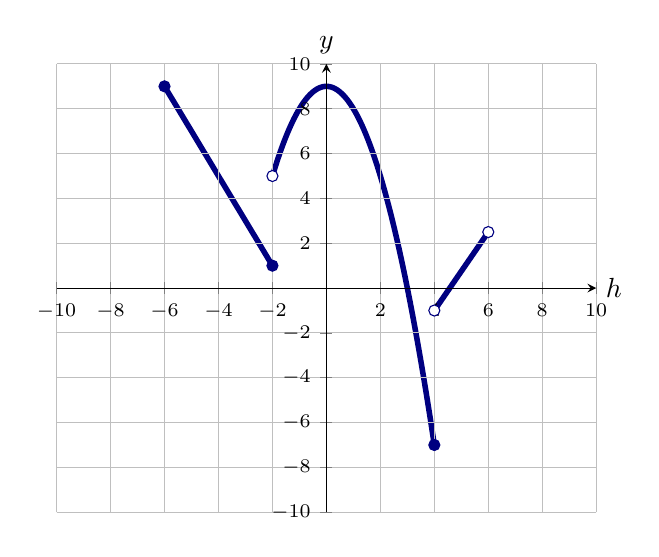
\begin{tikzpicture} 
  \begin{axis}[
            domain=-10:10, ymax=10, xmax=10, ymin=-10, xmin=-10,
            axis lines =center, xlabel=$h$, ylabel=$y$, grid = major,
            ytick={-10,-8,-6,-4,-2,2,4,6,8,10},
            xtick={-10,-8,-6,-4,-2,2,4,6,8,10},
            ticklabel style={font=\scriptsize},
            every axis y label/.style={at=(current axis.above origin),anchor=south},
            every axis x label/.style={at=(current axis.right of origin),anchor=west},
            axis on top
          ]
          
			\addplot [line width=2, penColor, smooth,samples=100,domain=(-6:-2)] {-2*x-3};
       		\addplot [line width=2, penColor, smooth,samples=100,domain=(-2:4)] {-1*(x+3)*(x-3))};
       		\addplot [line width=2, penColor, smooth,samples=100,domain=(4:6)] {1.75*x-8};




			\addplot[color=penColor,fill=penColor,only marks,mark=*] coordinates{(-6,9)};
			\addplot[color=penColor,fill=penColor,only marks,mark=*] coordinates{(-2,1)};

			\addplot[color=penColor,fill=white,only marks,mark=*] coordinates{(-2,5)};
			\addplot[color=penColor,fill=penColor,only marks,mark=*] coordinates{(4,-7)};

			\addplot[color=penColor,fill=white,only marks,mark=*] coordinates{(4,-1)};
			\addplot[color=penColor,fill=white,only marks,mark=*] coordinates{(6,2.5)};


           

  \end{axis}
\end{tikzpicture}
\end{image}




\subsection*{Domain} 

From the definition of $V(h)$, we can see the domain is $[-6, -2] \cup (-2, 4] \cup (4,6) = [-6, 6)$.



\subsection*{Zeros} 

We can see from the graph that usually the component pieces of $V$ would total four intercepts and zeros. One each from the linear pieces and two from the quadratic piece.  However, the domain restrictions only admit two of them.  The greater zero from the quadratic piece and the zero from the right linear function. These are both represented by intercepts on the graph.

The left line would have an intercept, except the domain does not allow it for $V$.  The middle parabola has a left intercept, except the domain does allow it for $V$. 

From the graph, we might estimate our two zeros to be around $3$ and $4.5$.  What are the exact values?







$\blacktriangleright$ The middle piece. 


\begin{explanation}


We are solving $-(h+3)(h-3) = 0$.  Since this is in factored form, we can quickly see the candidates are $-3$ and $3$.  $\answer{-3}$ is not in the domain for this piece of $V$, which is $(-2, 4]$.

Therefore, $V$ has $\answer{3}$ as its only zero contributed from the quadratic piece.
\end{explanation}



$\blacktriangleright$ The right piece. 


\begin{explanation}


We are solving $\frac{7h}{4} - 8 = 0$.  This give $\frac{32}{7}$ as a zero of $V$, which agrees with our extimation from the graph.

\end{explanation}













\subsection*{Continuity} 


Linear and quadratic functions are continuous functions. They are continous on restricted domains, which is what we have with piecewise defined functions.  $V(h)$ is continuous on $[-6, -2]$, $(-2, 4]$, and $(4, 6)$.  These correspond to the intervals in the definition of $V(h)$. \\

Therefore, we only need to check the endpoints of the intervals.  Here, those endpoints would be $\{ -6, -2, 4, 6 \}$.



\begin{observation} 
From the graph, we can see that 

\begin{itemize}
\item $-6$ is an included endpoint.  
\item there is a jump discontinuity at $-2$.
\item there is a jump discontinuity at $4$.
\item $6$ is not in the domain. It is an excluded endpoint.
\end{itemize}



\end{observation}


This will help direct our algebraic explanations. \\


The graph is suggesting that $-2$ and $4$ are discontinuities.  We have an algebraic definition for discontinuities.  Let's see if these domain numbers satisfy the definition. \\






\begin{explanation} Discontinuity at $-2$


Let $\epsilon > 0$ be any very small positive number.  Consider the corresponding interval, $(-2 - \epsilon, -2 + \epsilon)$.

\begin{itemize}
\item On $(-2 - \epsilon, -2)$, the values of $V$ are near $1$. \\

\begin{itemize}
  \item This is because $V$ is a linear function on $[-6, -2]$.
  \item $V$ is decreasing on $[-6, -2]$, because its formula has a negative leading coeffcient.
\end{itemize}

$V(h)$ is decreasing on $[-6, -2]$. \\
Which means $V(-6) >= V(a) >= V(b) >= V(-2)$ for all $a < b \in [-6, -2]$ \\

Let's select $a = -2 - \epsilon$ and $b = -2$. \\

\[
V(-2 - \epsilon) = -2 (-2 - \epsilon) - 3 = 4 + 2 \epsilon - 3 = 1 + 2 \epsilon 
\]

\[
V(-2) = 1
\]


Remember, $\epsilon$ is a very small postive number.  Certainly, $\epsilon < \frac{1}{2}$, so for sure $1 + 2 \epsilon < 2$. \\


\textbf{\textcolor{blue!55!black}{$\blacktriangleright$}} On $(-2 - \epsilon, -2)$, $2 >= V(h) >= 1$.

Now for the other side. \\



\item On $(-2, -2 + \epsilon)$, the values of $V$ are not near $2$.  They are around $7$. Let's verify this algebraically. \\



On this interval, $V(h) = 9 - h^2$. It is a quadratic function.  And, from the graph, it looks like $V \approx 7$ on this interval. How do we say this algebraically?  \\


Let's think for a moment.  If $V(h) = -(h + 3)(h - 3) = 9 - h^2$ was going to be near $2$, then we would need $h \approx -\sqrt{7}$.  \\

But, $-\sqrt{7} \notin (-2, -2 + \epsilon)$, since $-\sqrt{7} < -2$.  \\

\textbf{Note:} $h \approx \sqrt{7}$ would also make $V$ near $2$, but $\sqrt{7} \notin (-2, -2 + \epsilon)$, since the interval only contains negative numbers.\\

Let's glue this all together with algebraic and function reasoning. \\





\begin{itemize}
  \item $V$ is a quadratic function on $(-2, -1]$. 
  \[
V(h) = -(h + 3)(h - 3) = -h^2 -9
  \]
  \item The critical number of $V$ is $\frac{-b}{2a} = \frac{0}{-2} = 0$.
  \item $V$ is increasing on $(-2, -1]$, because its formula has a negative leading coeffcient and we are considering numbers less than $0$.
\end{itemize}

$V(h)$ is increasing on $(-2, -1]$. \\
Which means $V(a) <= V(b) <= V(-1)$ for all $a < b \in (-2, -1]$ \\

Let's select $a = -2 + \epsilon$ and $b = -1$. \\

\[
V(-2 + \epsilon) = -(-2 + \epsilon + 3) (-2 + \epsilon - 3) = -(1 + \epsilon) (-5 + \epsilon) = (1 + \epsilon) (5 - \epsilon)
\]

\[
V(-1) = 8
\]


Remember, $\epsilon$ is a very small postive number.  Certainly, $\epsilon < \frac{1}{2}$, so for sure  \\


\[
1 + \epsilon >= 1
\]

\[
5 -  \epsilon >= 5 -  \frac{1}{2} = \frac{9}{2}
\]




\textbf{\textcolor{blue!55!black}{$\blacktriangleright$}} On $(-2, -2 + \epsilon)$, we have


\[
V(h) >= 1 \cdot \frac{9}{2} = \frac{9}{2}
\]



On $(-2, -2 + \epsilon)$, we have $V(h) >=  \frac{9}{2}$.




\end{itemize}



\textbf{\textcolor{red!90!darkgray}{$\blacktriangleright$}} On $(-2 - \epsilon, -2)$, $2 >= V(h) >= 1$. \\

\textbf{\textcolor{red!90!darkgray}{$\blacktriangleright$}} On $(-2, -2 + \epsilon)$, we have $V(h) >=  \frac{9}{2}$. \\




Following the definition of discontinuity, let's pick a distance of $1$.


No matter how small $\epsilon$ is, $(-2 - \epsilon, -2 + \epsilon)$ \textbf{\textcolor{red!90!darkgray}{ALWAYS}} contains a domain number, $a \in (-2, -2 + \epsilon)$, such that the distance between $V(a)$ and $V(-2)$ is greater than $1$.

This tells us that there is a discontinuity at $-2$.

\end{explanation}








\begin{idea}


We are trying to get away from specific numbers. \\

We are trying to think of types of numbers. \\

We are trying to think of ``types'' as algebraic conditions or relationships. \\


This part of our new way of thinking.  We are trying to get away from specific numbers and, instead, think of \textbf{types} of numbers.  Our first encounter with this type of thinking is $\epsilon$.  It is representing a very small type of number, much smaller than the usual small numbers we have encountered in the past.  But, it is not any particular small number.  It is representing all of them. Kind of weird. \\


But, we need better language and notation to talk about discontiuities. \\

It is coming. \\

Limits will replace a lot of this kind of explanation. \\

Instead of talking about $\epsilon$, we will use limit notation to talk about expected values. \\

\[
\lim\limits_{h \to -2^+} V(h) = 7
\]

FOr now, we are figuring out how to talk about ``small'' numbers. \\

\end{idea}









\begin{explanation} Discontinuity at $4$


Let $\epsilon > 0$ be a small positive number.  Consider the corresponding interval, $(4 - \epsilon, 4 + \epsilon)$.

\begin{itemize}
\item On $(4 - \epsilon, 4)$, the values of $V$ are less than $-6$.
\item On $(4, 4 + \epsilon)$, the values of $V$ are greater than $-2$.
\end{itemize}


Following the definition of discontinuity, let's pick a distance of $1$.


No matter how small $\epsilon$ is, $(4 - \epsilon, 4 + \epsilon)$ \textbf{\textcolor{red!90!darkgray}{ALWAYS}} contains (at least) one domain number, $a \in (4, 4 + \epsilon)$, such that the distance between $V(a)$ and $V(4)$ is greater than $1$.

This tells us that there is a discontinuity at $4$.

\end{explanation}




\begin{notation}


Graphs are inherently inaccurate.  We cannot be exact with them.  They hide stuff all of the time. We need better ways, algebraic ways, of talking about types of discontinuities: ``jump'', ``removeable'', and ``asymptotic''.

Our algebraic notation to talk about function behavior around discontinuities and singularities will be called \textbf{\textcolor{purple!85!blue}{limits}}.  Limits have already made an appearance helping us describe end-behavior, algebraically.
\end{notation}










\subsection*{End-Behavior} 


End-behavior describes what the funciton is doing out in the ``tails'' of the domain.  But, here, the domain of $V$ is bounded.  There are no tails. \\

$V$ has no end-behavior. \\









\subsection*{Behavior : Increasing and Decreasing} 



\begin{itemize}
\item \textbf{$-2h-3$} is a linear function.  Its constant rate of change is $-2$.  This tells us it is a decreasing function.  $V$ is decreasing on $[-6, -2]$.

\item \textbf{$-(h+3)(h-3)$} is a quadratic on $(-2, 4]$. Here, $iRoC_V(h) = -2h$. The critical number occurs when $iRoC_V(h) = -2h = 0$, which happens when $h=0$. This agrees with the midpoint of the zeros, which are $-3$ and $3$.  Therefore, $0$ is where the function switches behavior.  

\begin{itemize}
\item On $(-2, 0)$, $iRoC_V(h) = -2h > 0$, therefore, $V$ is increasing.  
\item On $(0,4)$, $iRoC_V(h) = -2h < 0$, therefore, $V$ is decreasing.
\end{itemize}

This agrees with the graph.

\end{itemize}


\textbf{Technically:} We also need to account for the endpoints. $V$ is increasing on $[-2, 4]$, since the dot at $-2$ is lower than the left side of the included parabola.


\begin{question}
\begin{itemize}
\item \textbf{$\frac{7h}{4} - 8$} is a linear function with a constant rate of change of $\answer{\frac{7}{4}}$ telling us that $V$ is \wordChoice{\choice[correct]{increasing} \choice{decreasing}} on $(4, 6)$.
\end{itemize}
\end{question}

\textbf{Technically:} $V$ is increasing on $[4, 6)$, since the dot at $4$ is lower than the left side of the included line segment.


The intervals where $V$ is monotonic (always increasing or always decreasing) are

\begin{itemize}
\item $V$ is decreasing on $[-6,-2]$.
\item $V$ is increasing on $[-2,0]$.
\item $V$ is decreasing on $[0,4]$.
\item $V$ is increasing on $[4,6)$.
\end{itemize}









\subsection*{Extreme Values} 


We have three pieces to our function and the graph will help our algebra. We'll gather information about the pieces individually and then combine them for $V$.

\begin{itemize}
  \item \textbf{$-2h-3$} is a decreasing linear function on $[-6, -2]$.  Its maximum would occur at the left endpoint, which is included. Therefore, the maximum is $-2(-6)-3 = 9$. Its minimum would be at the right endpoint, which is included. Therefore, the minimum is $-2(-2)-3 = 1$.

  \item \textbf{$-(h+3)(h-3)$} is a quadratic on $(-2, 4]$.  Its graph is a parabola opening down and we have seen that $V$ increases and then decreases.  

  Therefore, its maximum value corresponds to the vertex, $(0, 9)$, which is included.  We get a maximum value of $9$.  The candidates for minimum value would occur at the endpoints, except only the right endpoint is included.  $-(4-3)(4+3) = -7$ is a possible minimum value.


\begin{observation}


We could have expanded the factored form: $-(h+3)(h-3) = -h^2 + 9$.  This is now in vertex form, $-(h-0)^2 + 9$. From this expression we can see that the vertex is $(0, 9)$, and the negative leading coefficient tells us that we have a maximum of $9$ occuring at $0$.


We could have observed the expanded form as a standard form, $-h^2 + 0 h + 9$.  Then the quadratic formula would give us $\frac{-b}{2a} = \frac{-0}{-2} = 0$ as the location of the vertex and the place where the behavior changes.


And, we can look at the instantaneous rate of change. The middle piece of $V$ is a quadratic, therefore, the vertex form $-(h-0)^2 + 9$ gives us $iRoC(h) = -2(h-0) = -2h$.  This equals $0$ at $0$, which means $0$ is a critical number and a possible location of changing behavior.

\end{observation}
Lastly, \\


  \item \textbf{$\frac{7h}{4} - 8$} is an increasing linear function on $(4, 6)$.  Its maximum would be encoded in the right endpoint, which is excluded. Its minimum would be encoded in the left endpoint, which is also excluded. This piece is contributing no extreme values to $V$.
\end{itemize}


Our analysis of the pieces leaves us with a global maximum value of $9$ for $V$.  $9$ occurs twice.  Once at $-6$ and then again at $0$.

Our analysis of the pieces leaves us with a global minimum value of $-7$ for $V$. $-7$ occurs once at $4$.



Each of these global extrema are also local extrema.  In addition we have $1$, which is a local minimum occuring at $-2$.  

\begin{explanation} Local Minimum


Consider the open interval $(-2 - 0.1, -2 + 0.1)$. $V$ is a decreasing function on $(-2 - 0.1, -2]$. $V$ is an increasing function on $[-2, -2 + 0.1)$.  This tells us that $V(-2)$ is a minimum value on this neighborhood of $-2$.  Thus, $V(-2) = 1$ is a local minimum of $V$.





\end{explanation}









\subsection*{Critical Numbers} 


$\blacktriangleright$ We know that the instantaneous rate of change of the middle quadratic is $iRoC_V(h) = -2h$ 

$\blacktriangleright$ We know that the instantaneous rate of change of the left linear is $iRoC_V(h) = -2$

$\blacktriangleright$ We know that the instantaneous rate of change of the right linear is $iRoC_V(h) = \frac{7}{4}$



The only place where the $iRoC_V(h) = 0$ is at $0$, therefore, $0$ is a critical number.


We also include domain numbers where the $iRoC_V$ does not exist.  That would be domain numbers where there is no corresponding tangent line.  That would include $-2$ and $4$.



The set of critical numbers is $\{ -2, 0, 4 \}$.




This doesn't include all of the places where we were investigating for extreme values. We also looked at $-6$.  There is a tangent line at $(-6, 9)$, which means $-6$ is not a critical number. Instead, $-6$ is an endpoint of a maximal interval of the domain. That automatically makes $-6$ a candidate for the location of an extreme value of $V$. \\


This also includes $-6$, becasue it is an endpoint of the domain. \\



Critical numbers and endpoints: $\{ -6, -2, 0, 4 \}$. \\

These are exactly the places we have been investigating for possible maximums and minimums.






\subsection*{Range} 


Since each piece of $V$ is continuous, the ranges of the three pieces of $V$ are $[1, 9]$, $[-7, 9]$, and $\left( -1, \frac{2}{5} \right)$. \\

The range of $V$ is their union.

\[
[1, 9] \cup [-7, 9] \cup \left( -1, \frac{2}{5} \right) = [-7, 9]
\]













\section*{Extrema : More Generally}


The extreme values of a function are the maximum and minimum values.  There are two types of each. \\

The global maximum and minimum values are the overall greatest and least values of the function.  There can be at most one global maximum value (there might not be an actual global maximum value). There can be at most one global minimum value (there might not be an actual global minimum value).  These two values can occur at many domain numbers.\\


Local maximum and minimum values are greatest and least values that occur in a ``neighborhood'' of a domain number.  There can be many local extrema values that occur at many domain numbers. \\


\begin{itemize}
\item Graphically, global maximum values are visually encoded as the highest point on the graph.
\item Graphically, global minimum values are visually encoded as the lowest point on the graph.
\item Graphically, local maximum values are visually encoded as the tops of hill on the graph.
\item Graphically, local minimum values are visually encoded as the bottoms of valleys on the graph.
\end{itemize}

also, \\

\begin{itemize}
\item Graphically, local extrema values can be visually encoded as endpoints.
\item Graphically, local extrema values can be visually encoded as singleton points.
\end{itemize}



\begin{template} \textbf{\textcolor{blue!55!black}{Extrema}} \\

As the function above illustrates, there are several places where extrema occur for functions.


\textbf{\textcolor{red!70!darkgray}{$\blacktriangleright$}} Horizontal Tangent Lines \\

An extreme value can occur where a tangent line is horizontal, or has a $0$ slope.  These would correspond to tops of hills and bottoms of valleys in the graph. \\




\textbf{\textcolor{red!70!darkgray}{$\blacktriangleright$}} Endpoints \\

Extreme values can happen at the endpoints. \\

\textbf{\textcolor{red!70!darkgray}{Peek Ahead:}} A graph can have a tangent line at an endpoint on a graph.  However, the derivative doesn't exist there since there is only one side.  In Calculus, we will talk about a one-sided derivative for these cases. \\

\end{template}




\begin{template} \textbf{\textcolor{blue!55!black}{Extrema}} \\

We have other places where an extreme value can occur. \\


\textbf{\textcolor{red!70!darkgray}{$\blacktriangleright$}} Vertical Tangent Lines \\

An extreme value can occur where a tangent line is vertical, or has no slope.  These would correspond to cusps in the graph. \\









\begin{image}
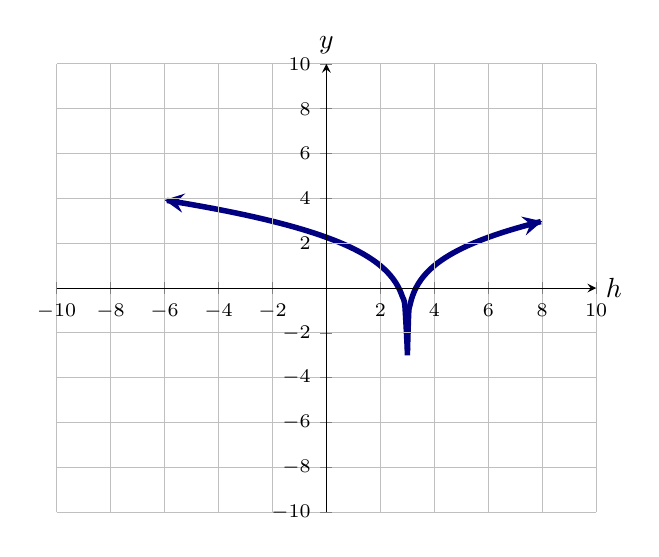
\begin{tikzpicture} 
  \begin{axis}[
            domain=-10:10, ymax=10, xmax=10, ymin=-10, xmin=-10,
            axis lines =center, xlabel=$h$, ylabel=$y$, grid = major,
            ytick={-10,-8,-6,-4,-2,2,4,6,8,10},
            xtick={-10,-8,-6,-4,-2,2,4,6,8,10},
            ticklabel style={font=\scriptsize},
            every axis y label/.style={at=(current axis.above origin),anchor=south},
            every axis x label/.style={at=(current axis.right of origin),anchor=west},
            axis on top
          ]
          
          \addplot [line width=2, penColor, smooth,samples=100,domain=(-6:3),<-] {4*(3-x)^(1/4)-3};
          \addplot [line width=2, penColor, smooth,samples=100,domain=(3:8),->] {4*(x-3)^(1/4)-3};

       

  \end{axis}
\end{tikzpicture}
\end{image}


This graph has a tangent line at $(3, -3)$.  It is a vertical line and vertical lines do not have a slope. \\









\textbf{\textcolor{red!70!darkgray}{$\blacktriangleright$}} Corners \\

An extreme value can occur where no tangent line exists.  These would correspond to corners in the graph. \\









\begin{image}
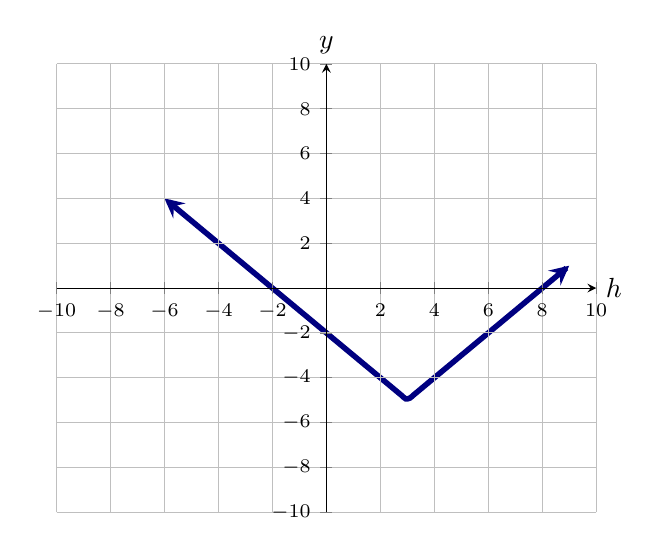
\begin{tikzpicture} 
  \begin{axis}[
            domain=-10:10, ymax=10, xmax=10, ymin=-10, xmin=-10,
            axis lines =center, xlabel=$h$, ylabel=$y$, grid = major,
            ytick={-10,-8,-6,-4,-2,2,4,6,8,10},
            xtick={-10,-8,-6,-4,-2,2,4,6,8,10},
            ticklabel style={font=\scriptsize},
            every axis y label/.style={at=(current axis.above origin),anchor=south},
            every axis x label/.style={at=(current axis.right of origin),anchor=west},
            axis on top
          ]
          
          \addplot [line width=2, penColor, smooth,samples=100,domain=(-6:9),<->] {abs(x-3) - 5};


       

  \end{axis}
\end{tikzpicture}
\end{image}


This graph has no tangent line at $(3, -5)$. 







\end{template}



We can sum up this ideas as follow: \\




\begin{center}


\textbf{\textcolor{red!70!darkgray}{Candidates for locations of extrema values are domain numbers where the derivative is $0$ or Does Not Exist.}}


\end{center}
















\begin{center}
\textbf{\textcolor{green!50!black}{ooooo-=-=-=-ooOoo-=-=-=-ooooo}} \\

more examples can be found by following this link\\ \link[More Examples of Piecewise-Defined Functions]{https://ximera.osu.edu/csccmathematics/precalculus1/precalculus1/piecewiseAnalysis/examples/exampleList}

\end{center}





\end{document}
